\subsubsection{Scénario Cockburn}
\textbf{Cas d'utilisation:} Payer par carte bleue

\textbf{Acteur primaire:} Le conducteur

\textbf{Pré-condition: } Le conducteur insère sa carte bleue dans la borne.

\textbf{Post-condition: }  La transaction a été validé ou pas.


\textbf{Scénario primaire: } \\
    \textbf{1.} Le lecteur de carte analyse la  carte bleue : la carte n’est pas une carte volée.\\ 
    \textbf{2.} La borne accepte le transaction(paiement). \\
  
\textbf{Variantes:}\\
    \textbf{1a1.} La vérification auprès des cartes volées indique que la carte bleue est volée.\\
    \textbf{1a2.} La transaction est échoue(payement est refusé). Fin scénario.\\
    
\newpage
\subsubsection{Diagramme d'activité}
\begin{figure}[h]
    \centering
    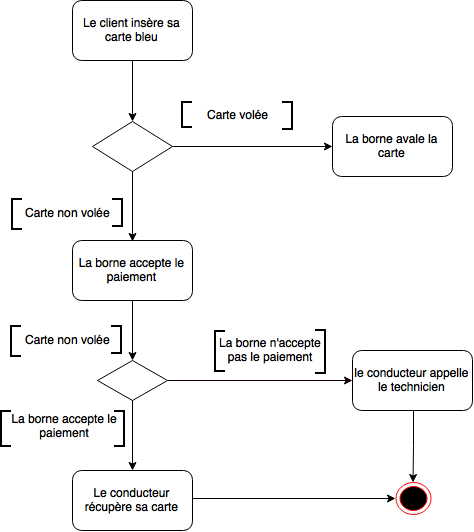
\includegraphics[scale=0.8]{02_Desenvolvimento/TD2/images/DAPayeBleu.png}
    \caption{Diagramme d'activité: Payer par carte bleue}
\end{figure}
\newpage
\subsubsection{Collaboration}
\begin{figure}[h]
    \centering
    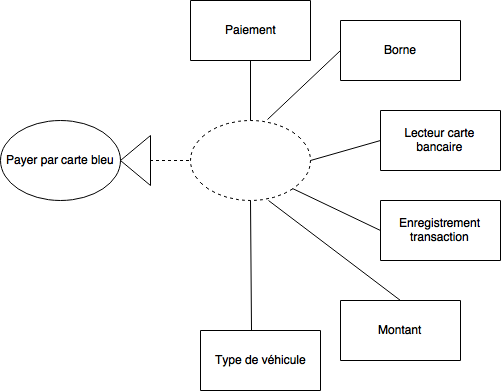
\includegraphics[scale=0.6]{02_Desenvolvimento/TD2/images/ColaCarteBleu.png}
    \caption{Collaboration: Payer par carte bleue}
\end{figure}
\newpage    
\subsubsection{Diagramme de séquence}
\begin{figure}[!htb]
    \centering
    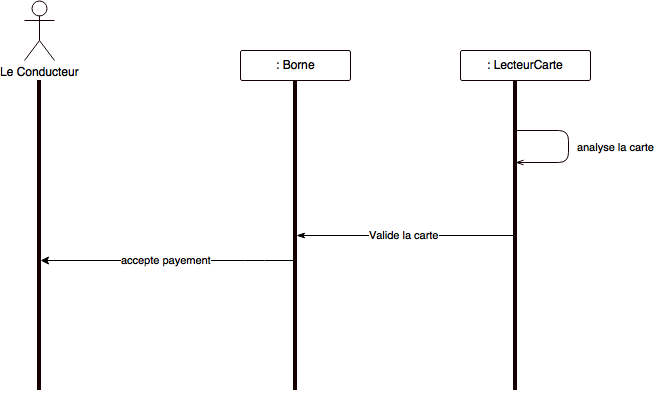
\includegraphics[scale=0.5]{02_Desenvolvimento/TD2/images/DS-payerCarteBleu.png}
    \caption{Diagramme de séquence - Payer par carte bleue - à revisiter }
\end{figure}
\subsubsection{Diagramme de séquence}
\begin{figure}[!htb]
    \centering
    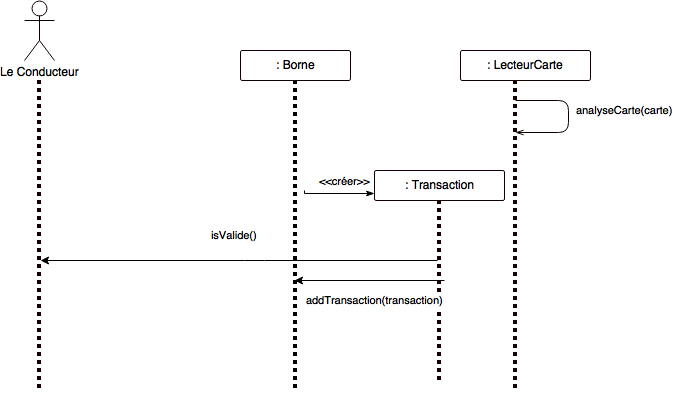
\includegraphics[scale=0.5]{02_Desenvolvimento/TD2/images/v2-DS-payerCarteBleu.png}
    \caption{Diagramme de séquence - Payer par carte bleue}
\end{figure}